\documentclass[sigconf]{acmart}
\usepackage{graphicx}
\usepackage{algorithmic}
\usepackage{algorithm}

%% Rights management information.  This information is sent to you
%% when you complete the rights form.  These commands have SAMPLE
%% values in them; it is your responsibility as an author to replace
%% the commands and values with those provided to you when you
%% complete the rights form.
\setcopyright{acmlicensed}
\copyrightyear{2025}
\acmYear{2025}
\acmConference[Algorithms Conference '25]{Proceedings of the Algorithms Conference '25}{May 20-June 3,
  2025}{Ljubljana, Slovenia}
\acmISBN{978-1-4503-XXXX-X/25/05}
\acmDOI{10.1145/XXXXXXX.XXXXXXX}

\acmArticleType{Review}

\title{Verifying Groups in Linear Time}

\author{Vanja Stojanovi\'c}
\email{vs66277@student.uni-lj.si}
\authornote{Corresponding author.}
\affiliation{
  \institution{University of Ljubljana}
  \department{Faculty of Mathematics and Physics}
  \city{Ljubljana}
  \country{Slovenia}
}

\author{Bor Panger\v si\v c}
\affiliation{
  \institution{University of Ljubljana}
  \department{Faculty of Mathematics and Physics}
  \city{Ljubljana}
  \country{Slovenia}
}

%— Authors from FRI —%
\author{Pia Sotlar}
\affiliation{
  \institution{University of Ljubljana}
  \department{Faculty of Computer Science and Informatics}
  \city{Ljubljana}
  \country{Slovenia}
}

\author{Klemen Kav\v ci\v c}
\affiliation{
  \institution{University of Ljubljana}
  \department{Faculty of Computer Science and Informatics}
  \city{Ljubljana}
  \country{Slovenia}
}

\keywords{Groups, Computational group theory, Cayley tables}

\begin{abstract}
  \bfseries
  We explore the latest upper and optimal bounds on the problem of deciding 
  whether a given \(n \times n\) multiplication table is a Cayley multiplication table of a 
  finite group, presented in \cite{10756141} and its cofindings. Exploring the applications of
  this algorithm, such as in computational group theory software, coding theory \cite{zurekCodingTheory} etc.
  \normalfont
\end{abstract}


\begin{document}

\maketitle


\section{Introduction}
\subsection{Motivation}
Verifying whether a given multiplication table defines a \textbf{group} is a fundamental problem in computational algebra with applications in cryptography, error-correcting codes, and symbolic computation. The key challenge lies in efficiently checking the \textbf{associativity axiom}, which naively requires testing all possible triplets \((a, b, c)\) to ensure:
\[
(a \cdot b) \cdot c = a \cdot (b \cdot c).
\]
A brute-force approach would require \(O(n^3)\) time, which is impractical for large \(n\). While prior work has improved this to \(O(n^2 \log n)\) deterministically or \(O(n^2)\) probabilistically, the question remains: \textbf{Can we do better?}

\subsubsection*{Why Linear Time is Non-Obvious}
A natural hope might be that associativity could be verified in \textbf{subcubic (or even linear) time} by exploiting algebraic structure. However, as demonstrated by the following theorem:

\begin{theorem}[Local Non-Associativity]
On every set with at least 4 elements, there exists a binary operation that is associative everywhere except on one triplet.
\end{theorem}
\begin{proof}
Let \( S \) be a set with \( |S| \geq 4 \). Choose distinct elements \( a, u, v, w \in S \). Define a binary operation \( * \) on \( S \) as follows:
\[
x * y =
\begin{cases}
u & \text{if } x = a \text{ and } y = a, \\
v & \text{if } x = a \text{ and } y = u, \\
w & \text{otherwise}.
\end{cases}
\]
We claim \( * \) is associative except for the triplet \( (a, a, a) \).
\\
\textbf{Non-associativity at \( (a, a, a) \):}
\[
(a * a) * a = u * a = w, \quad \text{but} \quad a * (a * a) = a * u = v.
\]
Since \( w \neq v \), \( (a * a) * a \neq a * (a * a) \).
\\
\textbf{Associativity for all other triplets:}
\\
First, let's analyze LHS $=(x \ast y) \ast z$. Let $p_1 = x \ast y$.
\begin{itemize}
    \item If $(x,y) = (a,a)$, then $p_1 = u$. LHS $= u \ast z$.
    Since $u \neq a$, the pair $(u,z)$ is neither $(a,a)$ nor $(a,u)$. So, $u \ast z = w$ by definition (3).
    \item If $(x,y) = (a,u)$, then $p_1 = v$. LHS $= v \ast z$.
    Since $v \neq a$, the pair $(v,z)$ is neither $(a,a)$ nor $(a,u)$. So, $v \ast z = w$ by definition (3).
    \item If $(x,y) \neq (a,a)$ and $(x,y) \neq (a,u)$, then $p_1 = w$. LHS $= w \ast z$.
    Since $w \neq a$, the pair $(w,z)$ is neither $(a,a)$ nor $(a,u)$. So, $w \ast z = w$ by definition (3).
\end{itemize}
In all possible cases for $(x,y)$, LHS $=(x \ast y) \ast z = w$.
\\
Next, let's analyze RHS $= x \ast (y \ast z)$. Let $p_2 = y \ast z$.
\begin{itemize}
    \item If $(y,z) = (a,a)$, then $p_2 = u$. RHS $= x \ast u$.
    \begin{itemize}
        \item If $x = a$, this corresponds to the triplet $(a,a,a)$. As shown before, RHS $= a \ast u = v$.
        \item If $x \neq a$, the pair $(x,u)$ is not $(a,a)$ (since $x \neq a$) and not $(a,u)$ (since $x \neq a$). So, $x \ast u = w$ by definition (3).
    \end{itemize}
    \item If $(y,z) = (a,u)$, then $p_2 = v$. RHS $= x \ast v$.
    Since $v \neq a$ and $v \neq u$ (as $a,u,v,w$ are distinct), the pair $(x,v)$ cannot be $(a,a)$ (as $v \neq a$) and cannot be $(a,u)$ (as $v \neq u$). So, $x \ast v = w$ by definition (3).
    \item If $(y,z) \neq (a,a)$ and $(y,z) \neq (a,u)$, then $p_2 = w$. RHS $= x \ast w$.
    Since $w \neq a$ and $w \neq u$ (as $a,u,v,w$ are distinct), the pair $(x,w)$ cannot be $(a,a)$ (as $w \neq a$) and cannot be $(a,u)$ (as $w \neq u$). So, $x \ast w = w$ by definition (3).
\end{itemize}

\end{proof}

This construction shows that:
\begin{itemize}
    \item \textbf{A single inconsistency suffices to break associativity.}
    \item \textbf{No local or sparse testing suffices}—even if almost all triplets are associative, the operation may still fail to be a group.
\end{itemize}

\subsection{Problem Statement}
Cayley table describes a structure of a finite group. It arranges all possible products of all the group's elements in a square table. To build a Cayley table we are given a set S and a binary operation \(\cdot : S \times S \rightarrow S\). In case of (\(|S| = n\)), a Cayley table is represented by a \(n\times n\) table, where entry (i,j) is a result of a binary operation on element in row i and element in column j, which is also an element of set S.
To know if a table represents a Cayley table, three properties have to be satisfied:
\begin{enumerate}
    \item Existence of an identity element: \(e: e \cdot s = s \cdot e = s\) for every \(s \in S\).
    \item Existence of inverses: for each \(s \in S\), there exists \(h \in S\) such that \(s \cdot h = h \cdot s = e\).
    \item Associativity: \((a \cdot b) \cdot c = a \cdot (b \cdot c)\) for all \(a,b,c \in S\).
\end{enumerate}
So if we are given an \( n \times n \) multiplication table, the goal is to determine if it represents a valid group.

A simple example of a Cayley table is one for the group \(\{1,-1 \}\):
\begin{center}
\begin{tabular}{|c|c|c|}
\hline
$\times$ & 1 & $-1$ \\
\hline
1   & 1   & $-1$ \\
\hline
$-1$ & $-1$ & 1   \\
\hline
\end{tabular}
\end{center}

Some of the features of a Cayley table are:
\begin{itemize}
    \item Every row and column of the table should contain each element exactly once.
    \item The identity element should appear in every row and column exactly once and it should be "distributed" on the main diagonal.
    \item Each entry must also be a row/column label. Otherwise, the operation is not closed.
    \item In the table there should be one row in which the column labels appear in order, this indicates the presence of an identity element.
\end{itemize}

\subsection{Applications of the Finding and Usage of Cayley Tables}

Within computational group theory software, such as GAP and Magma, efficient Cayley table verification plays a foundational role.
These systems allow users to define finite groups by providing their Cayley tables.
Upon input, the software must verify if the given table adheres to the group axioms (closure, associativity, identity, and inverses)
before allowing further computations or analysis. 

For instance, if a user intends to find the subgroups, conjugacy classes, or
other properties of a group defined by its Cayley table, the system first needs to ensure that the input indeed represents a valid group. 
Efficient verification algorithms make this initial validation process practical, especially for groups of moderate size. 
Furthermore, while not the most scalable approach for very large groups, Cayley tables can be employed in group isomorphism 
testing, particularly for groups with a smaller number of elements \cite{williams2015group}.

Finite groups also play a role in coding theory, particularly in the construction of error-correcting codes. For example, cyclic codes have a close 
relationship with cyclic groups. The algebraic properties of the underlying group often determine the characteristics and error-correcting
capabilities of these codes. The study of perfect codes (subsets of a graph with specific distance properties relevant to error correction)
sometimes involves Cayley graphs of groups.

In such contexts, verifying the group structure ensures that the Cayley graph possesses
the intended properties necessary for code construction and analysis. Additionally, research explores the construction of generator
and parity check matrices for error-correcting codes directly from the Cayley tables of certain algebraic structures \cite{zurekCodingTheory}.

\subsection{Prior Work}
To satisfy the third property of Cayley tables (associativity) we would have to check all triples. So to check for associativity, or more precisely that for every \(a,b,c  \in S\) it holds that \((a\times b)\times c = a\times (b\times c)\) a brute force algorithm would require \(\Theta(n^3)\) time. Before the linear-time algorithm, two other methods for checking associativity were proposed.
\subsubsection{Light's \( O(n^2 \log n) \) deterministic method}
In 1949 Dr. F. W. Light noticed that we can check for associativity only for all triples a,b,c such that \(a,c \in S\) and \(b\in R\), where R is a set of generators of S. A generating set R is a set of elements from set S from which you can build all other elements in the set S with the use of group operation. 

For a finite set S and a binary operation \((\cdot)\) we can define two operations:

\[a * c = a\cdot(b\cdot c)\] and
\[a \circ c= (a\cdot b)\cdot c\]

Associativity holds in S if for every element \(b \in R\) the operations \(*\) and \(\circ\) coincide for all \(a,c \in S\). We can do this reduction because if every element in S can be written as a combination of generators from R, and associativity is preserved, it is enough to verify associativity only on elements from R.
The general idea is to construct the Cayley tables for both operations and see if they are the same.

This method reduces the number of checks needed compared to checking all the combinations, because it avoids redundant computations. It checks associativity in \(\mathcal{O}(n^2logn)\) for R size \(logn\) and all \(a,c \in S\).

\begin{figure}[H]
    \centering
    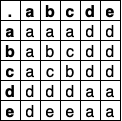
\includegraphics[width=0.125\linewidth]{original_table.png}
    \caption{Example table to demonstrate Light's associativity test}
\end{figure}

For table in Figure 1 \(\{c,e\}\) is the generating set. For c, the procedure is shown in Figure 2 below. We copy the c-row and c-column from the original table into new tables as the top and left headers. For each element in the header, we copy the corresponding column or row from the original table. To prove that associativity holds, we compare the *(c) and °(c) tables. If they are the same, associativity holds for c. Repeating this for all generators confirms associativity for the whole set.

\begin{figure}[H]
    \centering
    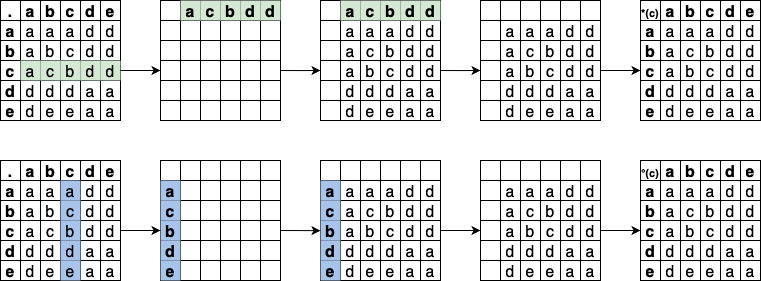
\includegraphics[width=0.5\linewidth]{Lights.png}
    \caption{Procedure for Light's associativity test}
\end{figure}

\begin{itemize}
    \item Brute-force: \( O(n^3) \) associativity checks.
    To satisfy the third property of Cayley tables (associativity) we would have to check all triples. So to check for associativity, or more precisely that for every \(a,b,c  \in S\) it holds that \((a\times b)\times c = a\times (b\times c)\) a brute force algorithm would require \(\Theta(n^3)\) time. Before the linear-time algorithm, two other methods for checking associativity were proposed.
    
    \item Light's \( O(n^2 \log n) \) deterministic method.

    
    \item Rajagopalan \& Schulman's randomized \( O(n^2 \log(1/\delta)) \).
    Rajagopalan and Schulman develop a randomized method, which achieves running time $O(n^2 \log(1/\delta))$, where $\delta$ is the allowed error probability. This reduces the time from cubic to nearly quadratic, making the approach much more efficient for large sets.
    Instead of checking all possible triplets in the set, the method randomly samples a carefully chosen number of triples and tests whether the associativity condition holds for each sampled combination. By choosing the number of samples carefully, they can detect non-associativity with high probability, even though they do not check every combination.
    The number of random samples $k$ is determined based on the desired error probability $\delta$:
    \[k = O\left(\frac{\log(1/\delta)}{\epsilon}\right).\]
    Here, $\epsilon$ is the (unknown) fraction of triples where associativity fails. 
    The method guarantees that if the operation is non-associative and enough triples fail, the probability of missing all failing triples after sampling is at most $\delta$. This makes the algorithm particularly useful when working with large data, where deterministic checking is computationally too expensive. It allows researchers to balance speed and confidence: they can choose the acceptable error $\delta$ and get a provably good result much faster than with deterministic methods.
    However, the efficiency depends on having a good understanding or estimate of the expected error $\epsilon$ in the table. If the number of failing triples is very small, the method may not be much more efficient than brute-force checking.
    Rajagopalan and Schulman’s method achieves complexity that is better than the one implied by Light’s observation when we allow a nonzero error probability $\delta$. However, the downside is that it does use randomness and introduces some probability of error.
    
\end{itemize}

\subsection{Contributions}
\begin{itemize}
    \item First deterministic \( O(n^2) \) algorithm.
    \item Use of \textbf{basis sets} and \textbf{4-associativity}.
    \item Reduction in the search for large subgroups by group decomposition.
\end{itemize}

\section{Technical Overview}
\subsection{Brute force methods}
When given a multiplication table (Cayley table) of a set $S$, we can check whether it has an identity element and inverses by brute force by systematically scanning the table. Each of these processes takes $O(n^2)$ time, where $n$ is the size of the set.

First, we check for the identity element. We need to find an element $e \in S$ that satisfies $e \cdot s = s \cdot e = s$ for all $s \in S$. To do this, we check for each element $s$ (candidate for $e$) all $n$ entries in row $e$ and all $n$ entries in column $e$ to see if they match the expected values. This gives $2n$ checks per candidate and $n$ candidates, for a total of $2n^2$ checks which gives us $O(n^2)$ complexity.

To check for inverses, we check for each element $s$ whether there exists an element $h$ such that $s \cdot h = h \cdot s = e$. We do this by scanning the row (or column) of $s$ to find a suitable $h$. This may require up to $n$ checks per $s$, and since there are $n$ elements $s$, this gives $n \times n = n^2$, which gives us $\to O(n^2)$ complexity.

By looping over all rows, columns, and element pairs, we can check identity and inverses in a group table using at most $O(n^2)$ operations — which is efficient compared to the associativity check, which typically requires $O(n^3)$ time. This is why the article focuses on improving the associativity check.

\subsection{Testing Group Axioms Efficiently}
\begin{itemize}
    \item Identity: Check \( \exists e \in G \) s.t. \( e \cdot g = g \cdot e = g \) (\( O(n) \)).
    Testing identity and inverse can be done more efficiently than just with a brute force method. 
    A method to find the identity in $O(n)$ time is to take any $ z \in S$ and multiply it with itself repeatedly. Since the group is finite, there exists $z^k = z^m$, where $k > m$. At this point, the elements start repeating. This happens after raising the element to the $n$-th power.    
    Once we find a repeat, we deduce that multiplying any element by $z^{k-m}$ returns the element itself, which makes it the identity element.
    We can take any element in $s \in G$:\[z^k \cdot s = z^m \cdot s\]
    \[z^{k-m} \cdot s = s\]
    \[z^{k-m}=e\]
    We then have to test the identity with all n elements so we can confirm that this holds for all elements. This takes another $2O(n)$ times (since we test \(e: e \cdot s = s \cdot e = s\) for every \(s \in S\)). 
    Using this approach we only performed an order on $n$ multiplications. $n$ multiplications for finding the $e$ and $2n$ for testing it. Overal this method for finding and checking the identity element runs in $O(n)$ time, which is significantly better than the brute force method that works in $O(n^2)$.
    
    \item Inverses: Find \( g^{-1} \) via exponentiation (\( O(n \log n) \)).
    From the method above we know that raising any element to the $n$th power yields the identity element $e$. Consequently, multiplying $s$ with itself $n-1$ times gives $s^{n-1}$, which serves as the inverse of $s$ because $s \cdot s^{n-1} = s^n = e$. From this we can say that $s^{-1} = s^{n-1}$
    So for finding the inverse we have to compute for each element $s \in S$ the value $s^{n-1}$. This runs in $O(\log n)$ steps for each element, giving the end complexity of $O(n\log n)$. We then check for each element that $s \cdot s^{-1} = e$. This time complexity is again much faster better than the brute force method $O(n^2)$.

    \item Example: Finding the Identity and Inverses in \( G = \{1, i, -1, -i\} \)
    Let \( G = \{1, i, -1, -i\} \) be a set under multiplication. We apply the efficient methods to find the identity and inverses.
  	\subsubsection*{Finding the Identity in \( O(n) \) Time}
    We pick an arbitrary element \( z \in G \). Let \( z = i \).
    We compute successive powers of \( i \) until a repetition occurs:
    \begin{align*}
    i^1 &= i \\
    i^2 &= -1 \\
    i^3 &= -i \\
    i^4 &= 1 \\
    i^5 &= i \quad (\text{repeat detected at } i^5 = i^1)
    \end{align*}
    We found a repeat at \( k = 5 \) and \( m = 1 \). According to the algorithm:\[e = i^{k - m} = i^{5 - 1} = i^4 = 1\]
    This means, the identity element is \( e = 1 \).
    Verification:\[1 \cdot g = g \cdot 1 = g \quad \forall g \in G\]
    We can see, that this holds for all elements:\[1 \cdot i = i,\quad 1 \cdot -1 = -1,\quad 1 \cdot -i = -i,\quad 1 \cdot 1 = 1\]
    \[i \cdot 1 = i, \quad -1 \cdot 1 = -1,\quad -i \cdot 1 = -i,\quad 1 \cdot 1 = 1\]
    This means, that \( e = 1 \) is confirmed as the identity.
    
    \subsubsection*{Finding Inverses via Exponentiation in \( O(n \log n) \) Time}
    We compute inverses using:\[g^{-1} = g^{n-1}\]
    where \( n = 4 \) (size of \( G \)).
    We calculate \( g^{-1} \) for each \( g \in G \):
    \begin{itemize}
      \item For \( g = 1 \):\[1^{-1} = 1^{3} = 1 \cdot 1 \cdot 1 = 1\]
      Verification:\[1 \cdot 1 = 1 = e\]
      \item For \( g = i \):\[i^{-1} = i^{3} = i \cdot i \cdot i = -i\]
      Verification:\[i \cdot -i = 1 = e\]
      \item For \( g = -1 \):\[(-1)^{-1} = (-1)^{3} = (-1) \cdot (-1) \cdot (-1) = -1\]
      Verification:\[-1 \cdot -1 = 1 = e\]
      \item For \( g = -i \):\[(-i)^{-1} = (-i)^{3} = (-i) \cdot (-i) \cdot (-i) = (-1) \cdot (-i) = i \]
      Verification:\[-i \cdot i = 1 = e\]
    \end{itemize}

  We successfully computed:\[e = 1\]
  \[1^{-1} = 1,\quad i^{-1} = -i,\quad -1^{-1} = -1,\quad -i^{-1} = i\] using \( O(n) \) operations to find the identity and \( O(n \log n) \) operations to compute inverses for all elements.
\end{itemize}

\subsection{4-Associativity and Basis Sets}
To verify if for a given operation on a set G is associative, many methods have been proposed. As mentioned a brute force approach requires \(\Theta(n^3)\) time. Light proposed a method that reduces the runtime to \(\mathcal{O}(n^2logn)\), while Rajagopalan and Schulman developed a randomized algorithm which achieves running time $O(n^2 \log(1/\delta))$. But, prior to this work, no other method has managed to reach lower running time than that.

\subsubsection{Basis and 4-associativity Definition}
Before we define and prove 4-associativity we first have to define the basis of a group.

If G is a set with a binary operation \(\cdot\): G×G→G, then a subset S of G is said to be a basis of G if $S\cdot S := \{s1\cdot s2 |s1,s2 \in S\}$ while $|S|\le3\sqrt{|G|}$.

The operation \(\cdot\) is said to be 4-associative over a set S, if for all $a,b,c,d \in S$ we have $((ab)c)d= (ab)(cd) = (a(bc))d= a((bc)d) = a(b(cd))$.

\subsubsection{Key Lemma}
If \(\cdot\) is 4-associative over S, then \(\cdot\) is associative over G.

\textbf{Proof}:
To prove 4-associativity over G, we first have to define \(\alpha, \beta,\gamma \in G\). So there exist elements \(a,b,c,d,e,f \in S\) such that
\[\alpha = ab,\]
\[\beta = cd,\]
\[\gamma = ef.\]


In order to show \( G \) is associative, we must prove
\begin{equation}
((ab)(cd))(ef) = (\alpha \cdot \beta) \cdot \gamma = \alpha \cdot (\beta \cdot \gamma) = (ab)((cd)(ef)). \tag{1}
\end{equation}

Since \( G = S \cdot S \), we can write
\[
b(cd) = uv, \quad a(uv) = wx, \quad (cd)e = st, \quad (st)f = pq, \quad (b(cd))e = yz,
\]
with \( p, q, s, t, u, v, w, x, y, z \in S \). Using this, and 4-associativity of \( \cdot \) on \( S \), we get that
\begin{align}
((ab)(cd))(ef) &= (a(b(cd)))(ef) = (wx)(ef) = ((wx)e)f \notag \\
&= ((a(uv))e)f = (a((uv)e))f = (a((b(cd))e))f. \tag{2}
\end{align}

Completely symmetrically, if we reflect all parentheses, we get
\begin{align}
(ab)((cd)(ef)) &= ab(((cd)e)f) = ab(pq) = a(b(pq)) \notag \\
&= a(b((st)f)) = a((b(st))f) = a((b((cd)e))f). \tag{3}
\end{align}

Finally, we show that the right-hand sides of (2) and (3) are equal, to deduce (1):
\[
(a((b(cd))e))f = (a(yz))f = a((yz)f) = a(((b(cd))e)f) = a((b((cd)e))f).
\]

Because we enumerate all sets of four elements of S ($|S| = O(\sqrt{n})$), we can check for 4-associativity in $\mathcal{O}\left((n^{1/2})^4\right) = \mathcal{O}(n^2)$ time.

\subsection{Reduction to Finding Large Subgroups}
\label{sec:large-subgroups}

%\subsubsection{Overview}
The core challenge in this subsection is constructing a \emph{basis} $S \subseteq G$ with $|S| = O(\sqrt{n})$ and $S^2 = G$, which enables efficient associativity testing via 4-associativity. The authors show that this reduces to finding \emph{large subgroups} $H \leq G$ where $|H| \geq \sqrt{|G|}$.

\begin{definition}[Large Subgroup]
A proper subgroup $H \leq G$ is \textbf{large} if $\sqrt{|G|} \leq |H| < |G|$.
\end{definition}

\begin{definition}[Group Decomposition]
For a group $G$ of size $n$ and parameter $\ell$, an \textbf{$\ell$-decomposition} is a pair $(A,B)$ where:
\begin{itemize}
    \item $A \cdot B = G$
    \item $|A| \leq 2\ell$
    \item $|B| \leq n/\ell$
\end{itemize}
\end{definition}

The reduction proceeds via three main phases:

\textbf{Phase 1: Recursive Decomposition}
Given a large subgroup $H$, we recursively decompose $G$:
\begin{itemize}
    \item \textbf{Base Case}: If $G$ is cyclic of prime order, use arithmetic progressions.
    \item \textbf{Recursive Case}:
    \begin{enumerate}
        \item If $|H| \geq n/(2\ell)$, set $A$ as a left transversal of $H$, $B = H$.
        \item Else, recursively decompose $H$ and lift to $G$ via transversals.
    \end{enumerate}
\end{itemize}

\begin{algorithm}[H]
\caption{GroupDecomposition}
\begin{algorithmic}[1]
%\Require Group $G$, parameter $\ell$
\IF{$|G|$ is prime}
    \STATE Return cyclic decomposition
\ELSE
    \STATE $H \gets \text{LargeSubgroup}(G)$
    \IF{$|H| \geq n/(2\ell)$}
        \STATE $A \gets \text{LeftTransversal}(G,H)$
        \STATE $B \gets H$
    \ELSE
        \STATE $(A',B') \gets \text{GroupDecomposition}(H,\ell)$
        \STATE $A \gets A'$
        \STATE $B \gets B' \cdot \text{RightTransversal}(G,H)$
    \ENDIF
\ENDIF
\RETURN $(A,B)$
\end{algorithmic}
\end{algorithm}

\textbf{Phase 2: Transversal Computation}
\begin{lemma}[Left Transversal]
A left transversal $T$ of $H \leq G$ can be found in $O(n)$ time by:
\begin{enumerate}
    \item Greedily selecting representatives from distinct cosets
    \item Removing entire cosets after selection
\end{enumerate}
\end{lemma}

\textbf{Phase 3: Basis Construction}
\begin{corollary}
Setting $\ell = \sqrt{n/2}$ yields a basis $S = A \cup B$ with $|S| \leq 2\sqrt{2n} < 3\sqrt{n}$.
\end{corollary}


\subsection{Reduction to Simple Groups}
\label{sec:simple-groups}

The algorithm reduces the large subgroup search problem to the case of \emph{simple groups} by:
\begin{itemize}
    \item Finding normal subgroups efficiently
    \item Recursively processing quotient groups
    \item Handling simple groups as base cases
\end{itemize}

\begin{definition}[Simple Group]
A group \( G \) is \textbf{simple} if its only normal subgroups are \( \{e\} \) and \( G \) itself.
\end{definition}

\subsubsection{Identifying normal subgroups}
The algorithm identifies normal subgroups through:

\textbf{Step 1: Small Generating Set}
\begin{itemize}
    \item Compute a generating set \( S \) with \( |S| \leq \log|G| \) in \( \widetilde{O}(n) \) time
    \item Uses greedy expansion of non-generator elements
\end{itemize}

\begin{algorithm}[H]
\caption{Generators}
\begin{algorithmic}[1]
\STATE \( H \gets \{e\} \)
\STATE \( S \gets \emptyset \)
\FOR{each \( a \in A \)}
    \IF{\( a \notin H \)}
        \STATE \( S \gets S \cup \{a\} \)
        \STATE \( H \gets \langle S \rangle \)
    \ENDIF
\ENDFOR
\RETURN \( S \)
\end{algorithmic}
\end{algorithm}

\textbf{Step 2: Conjugacy Class Graph}
\begin{itemize}
    \item Build graph where vertices are conjugacy classes
    \item Edge \( C_i \to C_j \) if elements from \( C_i \) multiply into \( C_j \)
    \item Compute in \( \widetilde{O}(n) \) time using generators
\end{itemize}

\textbf{Step 3: Closed Union Detection}
\begin{itemize}
    \item Normal subgroups correspond to closed unions of classes
    \item Dynamically maintain reachability in the graph
\end{itemize}

\subsubsection{Recursive Reduction}
\begin{lemma}[6.2]
Given an algorithm for simple groups, LargeSubgroup runs in \( O(n^{3/2+\epsilon}) \) time for arbitrary groups.
\end{lemma}

\begin{algorithm}[H]
\caption{LargeSubgroup}
\begin{algorithmic}[1]
\STATE \( N \gets \text{NormalSubgroup}(G) \)
\IF{\( N = G \)}
    \RETURN \(\text{LargeSubgroupOfSimpleGroup}(G)\)
\ELSIF{\( |N| \geq \sqrt{n} \)}
    \RETURN \( N \)
\ELSIF{\( G/N \) has prime order}
    \STATE Find element \( g \) of prime order \( p \)
    \RETURN \( \langle g \rangle \)
\ELSE
    \STATE \( M \gets \text{LargeSubgroup}(G/N) \)
    \RETURN \( M \cdot N \)
\ENDIF
\end{algorithmic}
\end{algorithm}

\subsubsection{Complexity Analysis}
\begin{itemize}
    \item Normal subgroup finding: \( \widetilde{O}(n) \) via dynamic graph maintenance
    \item Recursion depth: \( O(\log n) \) (each step reduces problem size)
    \item Bottleneck: Simple group handling (\( O(n^{3/2+\epsilon}) \))
\end{itemize}

\begin{theorem}
The reduction to simple groups preserves the overall \( O(n^{3/2+\epsilon}) \) time complexity when combined with:
\begin{itemize}
    \item \( \widetilde{O}(n) \) normal subgroup detection
    \item \( O(n^{3/2+\epsilon}) \) simple group processing
\end{itemize}
\end{theorem}

\subsection{Finding Large Subgroups of Simple Groups}
\label{sec:simple-subgroups}

The algorithm handles simple groups through a classification-based approach:

\begin{definition}[Simple Group Types]
Finite simple groups fall into three categories:
\begin{itemize}
    \item Cyclic groups of prime order
    \item Alternating groups $A_n$ ($n \geq 5$)
    \item Groups of Lie type and sporadic groups
\end{itemize}
\end{definition}

\subsubsection{Classification Strategy}
\begin{itemize}
    \item \textbf{Step 1: Group Identification} - Enumerate possible isomorphisms:
    \begin{algorithm}[H]
    \caption{EnumerateGroups}
    \begin{algorithmic}[1]
    \FOR{each simple group family $f$}
        \STATE Solve $|f(m,q)| = n$ for parameters $(m,q)$
        \IF{solution exists}
            \STATE Add $(f,m,q)$ to candidate list
        \ENDIF
    \ENDFOR
    \RETURN candidates
    \end{algorithmic}
    \end{algorithm}
    
    \item \textbf{Step 2: Type-Specific Handling} - Different approaches per category
\end{itemize}

\subsubsection{Algorithmic Approaches}

\textbf{Case 1: Alternating Groups ($A_n$)}
\begin{itemize}
    \item Find the natural subgroup $A_{n-1}$
    \item Implementation steps:
    \begin{enumerate}
        \item Identify all 3-cycles (elements of order 3)
        \item Find a set conjugate to $\{(1,2,k) | 3 \leq k \leq n\}$
        \item Remove one generator to get $A_{n-1}$
    \end{enumerate}
    \item Runtime: $\widetilde{O}(n)$
\end{itemize}

\textbf{Case 2: Groups of Lie Type}
\begin{itemize}
    \item Key tool: Borel subgroups
    \begin{definition}[Borel Subgroup]
    A maximal connected solvable subgroup.
    \end{definition}
    
    \item Implementation:
    \begin{algorithm}[H]
    \caption{BorelSubgroup}
    \begin{algorithmic}[1]
    \STATE Find Sylow $p$-subgroup $P$ (char. $p$ of field)
    \STATE Compute normalizer $B = N_G(P)$
    \RETURN $B$
    \end{algorithmic}
    \end{algorithm}
    
    \item Construct parabolic subgroup:
    \begin{itemize}
        \item Find element $a$ such that $P = \langle B, a \rangle$ is large
        \item Verify $|P| \geq \sqrt{|G|}$
    \end{itemize}
    \item Runtime: $O(n^{3/2+\epsilon})$
\end{itemize}

\textbf{Case 3: Sporadic Groups}
\begin{itemize}
    \item Finite list of 26 exceptions + Tits group
    \item Precomputed large subgroups from group theory literature
    \item Constant-time lookup
\end{itemize}

\subsubsection{Theoretical Guarantees}
\begin{theorem}[Existence]
Every non-prime simple group contains a large subgroup.
\end{theorem}

\begin{proof}[Proof Sketch]
\begin{itemize}
    \item Alternating: $|A_{n-1}| \geq \sqrt{|A_n|}$
    \item Lie type: Parabolic subgroups satisfy size requirement
    \item Sporadic: Verified case-by-case
\end{itemize}
\end{proof}

\subsubsection{Complexity Analysis}
\begin{itemize}
    \item Alternating groups: $\widetilde{O}(n)$ (dominated by 3-cycle detection)
    \item Lie type: $O(n^{3/2+\epsilon})$ (Borel subgroup construction)
    \item Sporadic: $O(1)$ (table lookup)
    \item Classification: $O(\log^4 n)$ (parameter solving)
\end{itemize}

\begin{lemma}
The simple group handling preserves the overall $O(n^{3/2+\epsilon})$ time complexity.
\end{lemma}

% 3. Critical Analysis (3–4 pages)
\section{Critical Analysis}
\subsection{Strengths}
\begin{itemize}
    \item Optimal complexity (\( \Omega(n^2) \) lower bound).
    \item Novel techniques: 4-associativity, group decomposition.
\end{itemize}

\subsection{Limitations}

\subsection{Open Problems}

% 4. Formalni dokazi (1–2 strani)
\section{Formal Proofs}
\subsection{4-Associativity Lemma}

\subsection{Existence of Large Subgroups}
Proof that non-prime finite groups have subgroups of size \( \geq \sqrt{n} \).

% 5. Conclusion (0.5–1 page)
\section{Conclusion}
Summary of results, implications for computational group theory, and future directions.

% References
\bibliographystyle{ACM-Reference-Format}
\bibliography{references}

\end{document}
